\documentclass{standalone}
\usepackage{tikz}
\usepackage{ctex,siunitx}
\setCJKmainfont{Noto Serif CJK SC}
\usepackage{tkz-euclide}
\usepackage{amsmath}
\usetikzlibrary{patterns, calc,3d}
\usetikzlibrary {decorations.pathmorphing,decorations.pathreplacing,decorations.shapes}
\tikzset{label style/.append style={font=\small}}
\begin{document}
\small
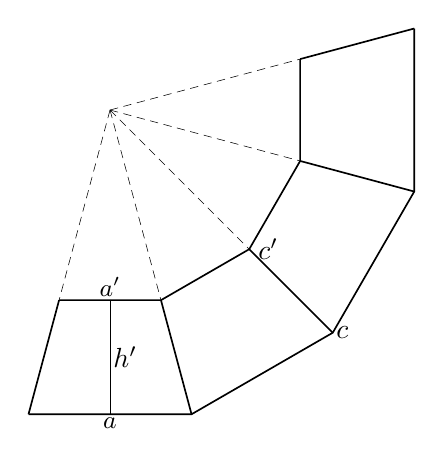
\begin{tikzpicture}[>=latex,scale=1.0,inner sep=1pt]
  \foreach \x in {-1,1,3,5,7}
  {
    \draw[very thin,densely dashed](0,0)--({270+\x*15}:2.5);
    \draw[semithick]({270+\x*15}:2.5)--({270+\x*15}:4);
  }
  \draw[semithick](255:2.5)--(285:2.5)--(315:2.5)node[right=2pt]{$c'$}--(345:2.5)--(375:2.5);
  \draw[semithick](255:4)--(285:4)--(315:4)node[right]{$c$}--(345:4)--(375:4);
  \tkzDefPoint(255:2.5){A'}
  \tkzDefPoint(285:2.5){B'}
  \tkzDefPoint(255:4){A}
  \tkzDefPoint(285:4){B}
  \tkzDefMidPoint(A,B)\tkzGetPoint{a}
  \tkzDefMidPoint(A',B')\tkzGetPoint{a'}
  \tkzDrawSegments(a,a')
  \tkzLabelLine[pos=0.5,right](a,a'){$h'$}
  \tkzLabelPoints[above](a')
  \tkzLabelPoints(a)
\end{tikzpicture}
\end{document}